\documentclass{report}\usepackage[]{graphicx}\usepackage[]{color}
%% maxwidth is the original width if it is less than linewidth
%% otherwise use linewidth (to make sure the graphics do not exceed the margin)
\makeatletter
\def\maxwidth{ %
  \ifdim\Gin@nat@width>\linewidth
    \linewidth
  \else
    \Gin@nat@width
  \fi
}
\makeatother

\definecolor{fgcolor}{rgb}{0.345, 0.345, 0.345}
\newcommand{\hlnum}[1]{\textcolor[rgb]{0.686,0.059,0.569}{#1}}%
\newcommand{\hlstr}[1]{\textcolor[rgb]{0.192,0.494,0.8}{#1}}%
\newcommand{\hlcom}[1]{\textcolor[rgb]{0.678,0.584,0.686}{\textit{#1}}}%
\newcommand{\hlopt}[1]{\textcolor[rgb]{0,0,0}{#1}}%
\newcommand{\hlstd}[1]{\textcolor[rgb]{0.345,0.345,0.345}{#1}}%
\newcommand{\hlkwa}[1]{\textcolor[rgb]{0.161,0.373,0.58}{\textbf{#1}}}%
\newcommand{\hlkwb}[1]{\textcolor[rgb]{0.69,0.353,0.396}{#1}}%
\newcommand{\hlkwc}[1]{\textcolor[rgb]{0.333,0.667,0.333}{#1}}%
\newcommand{\hlkwd}[1]{\textcolor[rgb]{0.737,0.353,0.396}{\textbf{#1}}}%
\let\hlipl\hlkwb

\usepackage{framed}
\makeatletter
\newenvironment{kframe}{%
 \def\at@end@of@kframe{}%
 \ifinner\ifhmode%
  \def\at@end@of@kframe{\end{minipage}}%
  \begin{minipage}{\columnwidth}%
 \fi\fi%
 \def\FrameCommand##1{\hskip\@totalleftmargin \hskip-\fboxsep
 \colorbox{shadecolor}{##1}\hskip-\fboxsep
     % There is no \\@totalrightmargin, so:
     \hskip-\linewidth \hskip-\@totalleftmargin \hskip\columnwidth}%
 \MakeFramed {\advance\hsize-\width
   \@totalleftmargin\z@ \linewidth\hsize
   \@setminipage}}%
 {\par\unskip\endMakeFramed%
 \at@end@of@kframe}
\makeatother

\definecolor{shadecolor}{rgb}{.97, .97, .97}
\definecolor{messagecolor}{rgb}{0, 0, 0}
\definecolor{warningcolor}{rgb}{1, 0, 1}
\definecolor{errorcolor}{rgb}{1, 0, 0}
\newenvironment{knitrout}{}{} % an empty environment to be redefined in TeX

\usepackage{alltt}
\usepackage{graphicx}

% Knitr environment configuration -------------------------------------
%% Knitr root folder - cannot run together with other chunks


%% Load the numbers from R cached results


\IfFileExists{upquote.sty}{\usepackage{upquote}}{}
\begin{document}

\title{A dynamic report}
\vskip 0.5cm
\author{Lingyun Zhang}


\vskip 0.3cm

\maketitle

\date{}

\section{Introduction}

This section should have the {\bf context} and ....

\section{Content}

In 2015, the total Ford US sales was {\bf 2,613,162} vehicles and the average sale was {\bf 217,764} vehicles per month ....

We insert a graph here:
\begin{figure}[htbp]
	\caption{Ford US monthly sales in 2015}
	\label{fig:001} 
	\centering 
	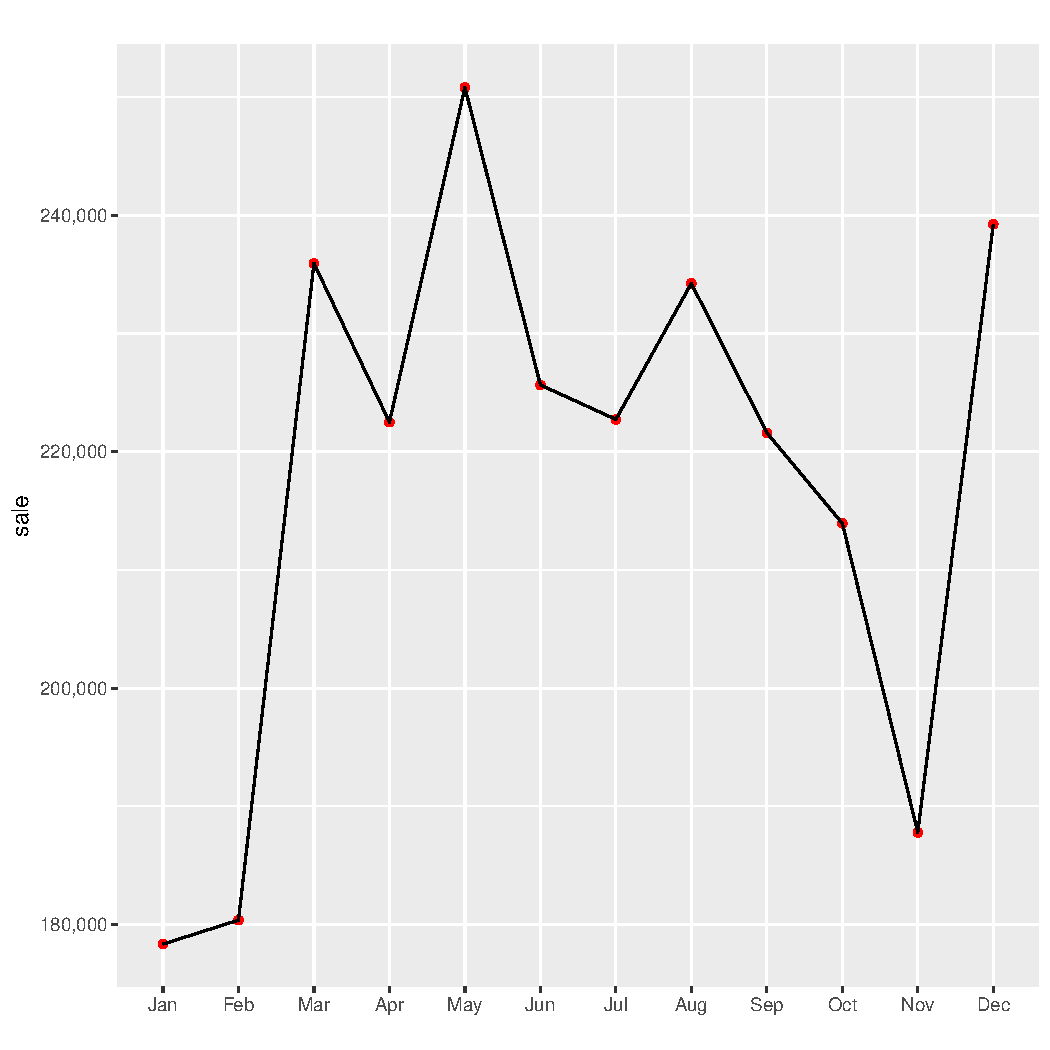
\includegraphics[scale=0.75]{../Figures/Ford_monthly_sale.pdf}
\end{figure}

\section{Conclusion}

We insert a table here:
% latex table generated in R 3.3.3 by xtable 1.8-2 package
% Fri Apr 14 20:56:49 2017
\begin{table}[h]
\centering
\caption{Ford US quarterly sales in 2015} 
\label{table1}
\scalebox{1}{
\begin{tabular}{cll}
  \hline
QuarterNumber & total & average \\ 
  \hline
1 & 594663 & 198221 \\ 
  2 & 698958 & 232986 \\ 
  3 & 678567 & 226189 \\ 
  4 & 640974 & 213658 \\ 
   \hline
\end{tabular}
}
\end{table}



\end{document}
